\documentclass{beamer}
\usetheme{Madrid}
\usepackage{xcolor}
\usecolortheme{whale}
\useoutertheme{miniframes} % Adds navigation dots

\title{Introduction to State Space Models}
\subtitle{UG BTech - 2nd Year}
\author{Vinay , Vaibhav Mahore , Shubhadeep Sing , Snehal Biswas}
\institute{Indian Institute of Science, Bangalore}
\date{\today}

\begin{document}

\frame{\titlepage}

\section{Outline}




\section{Introduction}

% Slide 1: Need for Sequential Data Modeling
\begin{frame}
\frametitle{The Need for Sequential Data Modeling}
\begin{itemize}
    \item \textbf{What is Sequential Data?}   \\
    \begin{itemize}
        \item \textbf{Ans :} It's the  data that comes in a specific order, where the arrangement of the data points matters.
    \end{itemize}
    \item \textbf{Example(NLP):}  
    The \textcolor{blue}{dog} bites the \textcolor{red}{man} vs The \textcolor{red}{man} bites the \textcolor{blue}{dog}.
    \item \textbf{Need for Sequential Data Modeling:}
    It's crucial because many datasets have an inherent order e.g Language, Time series in which the sequence and context between data points are essential for accurate analysis and predictions.
    \item \textbf{Challenge:}  
    Traditional models(e.g. Feedforward Networks) treat inputs independently and fail to capture such temporal dependencies.
\end{itemize}
\end{frame}

% Slide 2: RNN Basics
\begin{frame}
\frametitle{Recurrent Neural Networks (RNNs)}
    \begin{itemize}
        \item \textbf{Why RNNs?}
        \begin{itemize}
            \item A key characteristic that sets RNN apart from traditional FFN is their \textbf{recurrence}, which allows them to maintain an internal state over time .
                \end{itemize}
            \begin{figure}[h]  % 'h' suggests placing it here
                \centering
                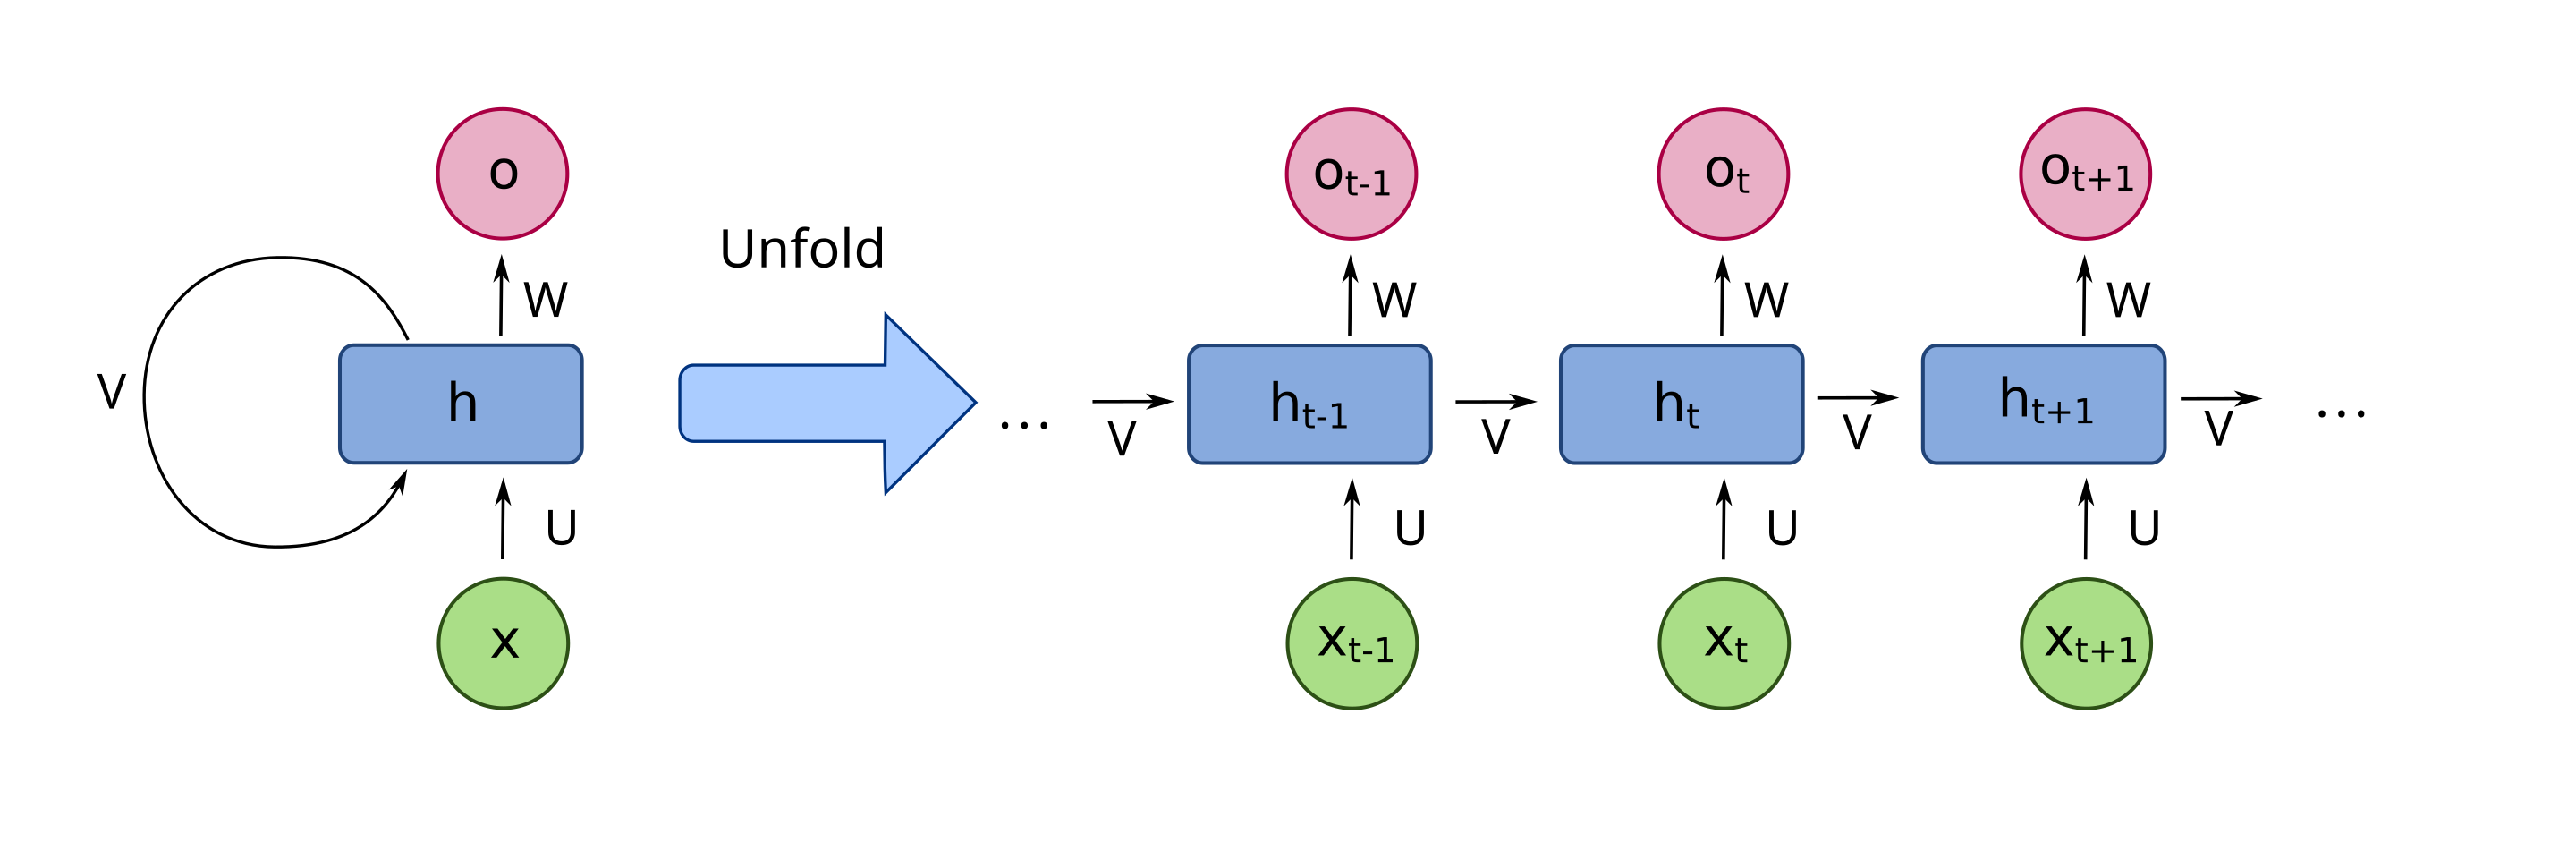
\includegraphics[width=0.8\textwidth]{RNN.png}
            \end{figure}     
            \begin{align}
            h_t &= \sigma(W_{hh} \cdot h_{t-1} + W_{xh} \cdot x_t + b_h) \\
            o_t &= W_{hy} \cdot h_t + b_y
        \end{align}
    \end{itemize}
\end{frame}
    
    
    
    %Slide 3: RNN Architecture and Limitations
    
\begin{frame}
\frametitle{RNNs: Structure and Challenges}
    \begin{itemize}
        \item \textbf{Benefits:}
        \begin{itemize}
            \item \textbf{Temporal Contextualization:} RNNs maintain an internal state that carries information from previous time steps, allowing them to capture the temporal dependencies inherent in sequential data.
            \item \textbf{Efficient Weight Sharing:} RNNs share weights across different time steps, reducing the number of parameters and improving generalization.
        \end{itemize}
        
        \item \textbf{Challenges:}
        \begin{itemize}
            \item \textbf{Vanishing and Exploding Gradients:}
            Gradients may decay over time making early data less influential or
            become excessively large leading to training instability.

           
            \item \textbf{Sequential Processing Bottleneck:}
            RNNs process data sequentially, making them computationally inefficient, especially for long sequences.
           
        \end{itemize}
    \end{itemize}
\end{frame}

% Slide 3: Transition from RNN to LSTM
\begin{frame}
    \frametitle{Long Short-Term Memory (LSTM)}
    \vspace{0cm}
    
    \begin{columns}[T]
        % Left Column
        \column{0.5\textwidth}
        \begin{itemize}
            \item \textbf{Introduction of LSTM:}
            \begin{itemize}
                \item LSTMs overcome standard RNN limitations by using a dedicated cell state to store and retain long-term information.
                \item They use three specialized gates—input, forget, and output—to precisely control how data enters and exits the cell state.
            \end{itemize}
        \end{itemize}

        % First part of the equations in small font size
        \vspace{-0.4cm}
        {\small
        \[
        \begin{aligned}
            f_t &= \sigma\bigl(W_f [h_{t-1}, x_t] + b_f\bigr),\\[5pt]
            i_t &= \sigma\bigl(W_i [h_{t-1}, x_t] + b_i\bigr),\\[5pt]
            \tilde{C}_t &= \tanh\bigl(W_C [h_{t-1}, x_t] + b_C\bigr),
        \end{aligned}
        \]
        }
        
        % Right Column
        \column{0.5\textwidth}
        \raggedright
        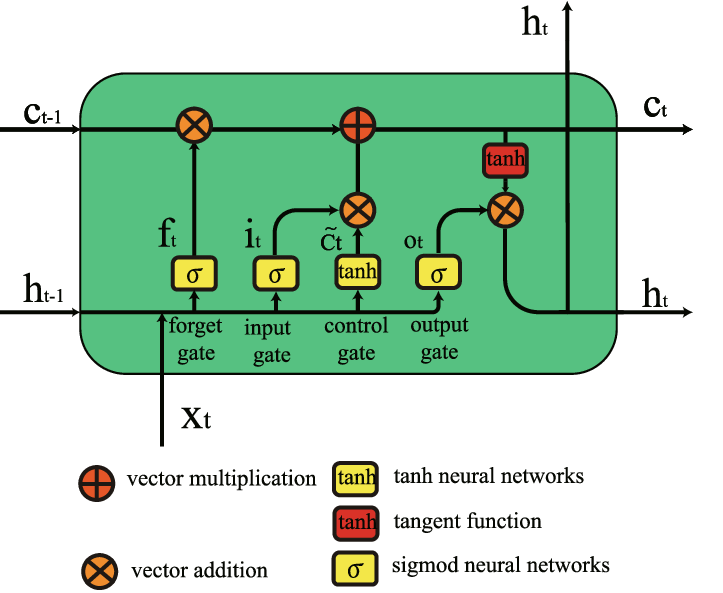
\includegraphics[width=0.9\textwidth]{LSTM.png}
        \vspace{-0.15cm}
        
        {\small
        \[
        \begin{aligned}
            C_t &= f_t \times C_{t-1} + i_t \times \tilde{C}_t,\\[5pt]
            o_t &= \sigma\bigl(W_o [h_{t-1}, x_t] + b_o\bigr),\\[5pt]
            h_t &= o_t \times \tanh\bigl(C_t\bigr).
        \end{aligned}
        \]
        }
    \end{columns}
\end{frame}
% Slide 4: Limitations of LSTM (with research backing)
\begin{frame}
\frametitle{Limitations of LSTMs}
\begin{itemize}
    \item \textbf{Scalability and Computational Complexity:}
    \begin{itemize}
        \item Despite improvements, LSTMs remain computationally intensive for very long sequences.
    \end{itemize}
    \item \textbf{Long-Range Dependency Challenges:}
    \begin{itemize}
        \item Research such as Bengio et al. (1994) and Pascanu et al. (2013) has demonstrated that LSTMs can still struggle with vanishing gradients when modeling very long sequences.
    \end{itemize}
    \item \textbf{Sequential Processing Bottleneck:}
    \begin{itemize}
        \item The inherent sequential nature of LSTM processing limits parallelism, resulting in slower training compared to more modern architectures.
    \end{itemize}
\end{itemize}
\end{frame}


\section{Methodology}
\begin{frame}
\frametitle{Methodology}
\begin{itemize}
    \item Data collection and preprocessing
    \item Model architecture
    \item Training approach
    \item Evaluation metrics
\end{itemize}
\end{frame}

\section{Implementation}
\begin{frame}
\frametitle{Implementation}
\begin{itemize}
    \item Technologies used
    \item Key algorithms
    \item Technical challenges
    \item Solutions implemented
\end{itemize}
\end{frame}

\section{Results}
\begin{frame}
\frametitle{Results}
\begin{itemize}
    \item Model performance
    \item Key findings
    \item Comparative analysis
    \item Visualizations
\end{itemize}
\end{frame}

\section{Future Work}
\begin{frame}
\frametitle{Future Work}
\begin{itemize}
    \item Potential improvements
    \item Scalability considerations
    \item Additional features
    \item Research directions
\end{itemize}
\end{frame}

\begin{frame}
\frametitle{Thank You}
\begin{center}
    any Questions?
\end{center}
\end{frame}

\end{document}
 